\documentclass[conference]{IEEEtran}
\IEEEoverridecommandlockouts

\usepackage{cite}
\usepackage{amsmath,amssymb,amsfonts}
\usepackage{algorithmic}
\usepackage{graphicx}
\usepackage{textcomp}
\usepackage{xcolor}
\usepackage{amsthm, hyperref, float}

\def\BibTeX{{\rm B\kern-.05em{\sc i\kern-.025em b}\kern-.08em
    T\kern-.1667em\lower.7ex\hbox{E}\kern-.125emX}}
\begin{document}

\title{Visual Place Recognition: Bag of Visual Words and Object Detection Extension\\
{\footnotesize \textsuperscript{*}Note: This is a final report for AER1515 course project}
}

\author{\IEEEauthorblockN{Zhenyuan Xiang}
\IEEEauthorblockA{\textit{Department of Electrical \& Computer Engineering} \\
\textit{University of Toronto}\\
Toronto, Canada \\
kelvin.xiang@mail.utoronto.ca}
\and
\IEEEauthorblockN{Zhentao Fan}
\IEEEauthorblockA{\textit{Department of Electrical \& Computer Engineering} \\
\textit{University of Toronto}\\
Toronto, Canada \\
zhentao.fan@mail.utoronto.ca}
}

\maketitle

\begin{abstract}
This report presents an enhanced method for visual place recognition (VPR) in the domain of computer vision, aiming to improve the accuracy of traditional bag-of-visual-words (BoVW) approaches. Our methodology integrates object recognition to identify the frequency vector of feature objects in a scene. These frequency vectors are then weighted and combined with the BoVW. Additionally, we discuss several other optimization methods to further refine our approach. Our primary discovery reveals a increase in accuracy, with an average improvement of approximately 1.4\%, even when recognizing a limited set of just five feature objects. Extensive random testing was conducted using the GSV-cities dataset\cite{ali2022gsv} to validate the effectiveness of our method. This enhanced VPR method has a wide range of potential application scenarios, especially in the field of autonomous driving and augmented reality (AR), where it can provide more reliable and simultaneously efficient service.
\end{abstract}

\begin{IEEEkeywords}
Visual place recognition, Bag of Visual Words, image classification, object detection
\end{IEEEkeywords}

\section{Introduction}

Visual Place Recognition (VPR) is a crucial component in the field of robotic perception. It's used to help computers and robots figure out where they are by looking at images of different places. This has strong implications in various cutting-edge applications like autonomous driving, robotic navigation, and augmented reality. VPR is also a challenging problem. In many cases, VPR models need to be able to handle dozens, hundreds, or even thousands of different locations. Also, variability in lighting, seasonal changes, and different viewpoints can drastically alter the appearance of a location in images, which significantly raises the difficulty of categorizing different places.

The Bag of Visual Words (BoVW) method, inspired by the Bag of Words method in natural language processing, is a notable approach to for image classification\cite{yang2010bag} and VPR. This method involves extracting features (i.e. SIFT) from images and representing them as a collection of ``visual words'', thereby transforming complex visual inputs into a simplified, yet effective, vector format for analysis. While BoVW has shown decent results in VPR, its performance still has potential for improvement. 

Considering that BoVW only extract simple features from images to construct its vocabulary and bag of words, an intuitive enhancement direction is to use deep learning methods to recognize representative feature objects in the scene, such as traffic lights, fire hydrants, etc., and put these significant features into the vocabulary. Another direction is to remove unrepresentative features from the image, i.e., detecting Region of Non-Interest (RoNI) in the input image. Using pretrained deep learning models like YOLOv3\cite{redmon2018yolov3} and YOLOv5, these enhancements can be implemented easily and efficiently.

This report discusses the implementation and fine-tuning of the traditional BoVW method, such as the setting of key parameters and the selection of classifiers, as well as the implementation of the two enhancements mentioned above and their performance. Through these, we hope to further improve the accuracy of our VPR model without significantly increasing the computational complexity.

\section{Related Work}

The field of visual place recognition (VPR) has been extensively explored, particularly focusing on improving accuracy and robustness of location recognition in diverse environments.

In order to recognize places regardless of the position and angle of the viewer, the BoVW method ignores the spatial information in the images\cite{lowry2015visual}. This improves the robustness of the model, but also means that it is not possible to discriminate between two places that are similar in features but have different spatial layouts. To address this problem, Y. Yang and S. Newsam\cite{yang2010bag} proposed spatial extensions to BoVW. In addition, the automatic BoVW method for online robot navigation and mapping, as described in the work by T. Nicosevici et al.\cite{nicosevici2012automatic}, can build and update the vocabulary continuously, without requiring training the BoVW model before robots entering the environment. These methods further enhance the potential of BoVW for practical applications.

In their survey, S. Lowry et al.\cite{lowry2015visual} mention that the use of global descriptors improves robustness to environment changes (e.g. different lighting conditions) compared to the use of local descriptors (e.g. SIFT). They also explained an example of extracting potential landmarks in the scene using the Box-Edge method proposed by C. L. Zitnick et al.\cite{zitnick2014edge}.

\section{Problem Definition}

\subsection{Input}

An image of a place that is captured by a camera: $x$.

\subsection{Output}

A label or a name of the place that the input image is taken: $s = M(x)$, where $M$ is the model.

\subsection{Domain \& Range}

Since our model uses offline method and requires prebuilt vocabulary, the output is limited to the places that we have collected and labeled in our training set. The input can be any image, but only the image taken from the location that has been collected and labeled would get a reasonable prediction.

\section{Baseline}

As mentioned earlier, we are using BoVW as our baseline model. We will briefly introduce our BoVW implementation in this section and discuss some details, such as the choice of parameters and classifiers.

\subsection*{Stage 1. Loading Images from the training set}

The process starts by reading the training set images and labels. The BoVW model does not have strict requirements on the size of the input images as it uses local descriptors. However, better results should be obtained when the images are of uniform size, as that guarantees the number of features that the image can contain. As an example, for the same location, a smaller image may contain fewer features, which can affect the accuracy of the classifier.

\subsection*{Stage 2. Feature Detection and Description}

We transformed each image into a grayscale image and computed their SIFT features using OpenCV. Then we save only the feature descriptors, ignoring the coordinates of the keypoints. To ensure performance, we limit the number of features per graph to 2,000. To ensure performance, we limit the number of features per graph to 2,000. Through experiments, we found that further increasing the number of features does not bring significant accuracy improvement, but only consumes more computational resources.

The reason why we choose to use SIFT as the feature detector includes:

\begin{itemize}
    \item Scale \& Rotation Invariance: SIFT features remain invariant to image scaling and rotation, which ensures that the same descriptors do not change as the observer's position in space changes.
    \item Robustness: SIFT features are very resistant to lighting variations, noise, and other small local variations in the image.
    \item Distinctive Descriptor: SIFT is able to describe the features in an image in detail (feature vectors of length 128), which facilitates us to classify similar features into the same cluster more accurately in the next step.
\end{itemize}

\subsection*{Stage 3. Building the Visual Vocabulary}

The descriptors from all images in the training set are then used to build a visual vocabulary. This is achieved through a clustering algorithm, which is k-means in our case. The descriptors are grouped into clusters, with each cluster representing a ``visual word''. The idea is to categorize similar features together, forming a dictionary of visual words. Similar descriptors are classified into the same word, just as different forms of the same word in a text version of BoW are considered to be the same word.

As for the choice of the number of clusters, we set it to 1,500 based on our experimental results. Considering that we set the number of features around 2,000, this value is reasonable because it ensures that the frequency vectors of each graph are ``sparse'', which helps to improve the accuracy of SVC. This parameter needs to be chosen carefully. If it is too small it can lead to different features being recognized as the same visual word, whereas if it is too large it can lead to same but slightly different features being recognized as completely different words (overfitting).

\subsection*{Stage 4. Quantization of Features}

Once the visual vocabulary is established, we can quantify the features in each image. For each image, we input its features detected in Stage 2 into our trained k-means model to obtain the frequency of each visual word (i.e., feature clusters). This effectively converts the image into a fixed-size vector, where each dimension represents a visual word, and the value in that dimension is the frequency of that word in the image.

\subsection*{Stage 5. Training the Classifier}

The learning methods we have used so far are unsupervised learning. Now, we have to use a supervised learning method, to enable our model to classify different locations. To do this, we tried two classic classifiers: Support Vector Classification (SVC) and random decision forests. The classifiers are trained with frequency vectors from training images, along with their location labels.

We tested SVC with a variety of kernels as well as the Random Forest method and found that SVC with a linear kernel had the best accuracy (about 10\% better than the other kernels and the Random Forest), so we adopted it in our implementation. This shows the good linear distinguishability of our extracted feature vectors. In addition, the other kernels of SVC do not perform as well as the linear kernel possibly due to overfitting.

\section{Object Detection Extension}

\subsection{Overview}

The BoVW method uses only local descriptors, thus the overall structural information of the object may be ignored. Inspired by S. Lowry et al.\cite{lowry2015visual}'s survey, we explored object detection extension to the BoVW method.

We believe that fusing object recognition as global descriptors with SIFT features can enhance the feature description capabilities. SIFT features are already effective in feature description. However, they primarily focus on local features and might overlook the overall structure of an object. Integrating object detection allows for a more comprehensive and accurate feature description that considers both local details and the overall structure of the object.

\subsection{Object Detection Using YOLOv5}

For object detection, we utilized the well-known YOLOv5 model. By loading the pre-trained model of YOLOv5 using PyTorch, we were able to recognize some of the objects in the scene very efficiently and accurately. More specifically, we chose YOLOv5x in our experiments, which is the most accuracy and complex one among all pre-trained YOLOv5 models, to ensure the model's accuracy.

However, since YOLOv5 is trained on Microsoft COCO\cite{lin2014microsoft} dataset, the objects that can be detected are limited. Among the objects included in the Microsoft COCO dataset, we chose the following five items:

\begin{verbatim}
    INTERESTING_OBJ_LIST = [
        'traffic light',
        'fire hydrant',
        'stop sign',
        'parking meter',
        'bench'
    ]
\end{verbatim}

These objects were selected because they are commonly found in urban environments and are relatively static and distinctive, making them excellent landmarks for place recognition.

Just like the original BoVW approach, we ignore the spatial information of the detected objects, and only store the frequency of each objects. In this way, we get another frequency vector.

\subsection{Fusion with SIFT features}

In order to integrate the baseline approach with the object detection extension, we chose a very intuitive approach: consider each object as a word and put it into the original vocabulary. In practice, we simply need to concatenate the frequency vector obtained from object detection with the SIFT frequency vector.

However, the change about by just concatenate only is negligible, considering that our object detection vectors have a length of only 5, whereas SIFT vectors have a length of up to 1,500. Since our object detection is highly accurate and better generalizes the overall properties of the feature objects in the image, we can make the frequencies of these objects have a greater impact on the SVC decision by multiplying a weight on the object frequencies.

The following figure \ref{fig:1} shows the structure of the BoVW method with object detection extension, where $\overrightarrow{v_1}$ is the SIFT frequency vector, $\overrightarrow{v_2}$ is the object detection vector, and $w$ is the weighting factor.

\begin{figure}[H]
    \centering
    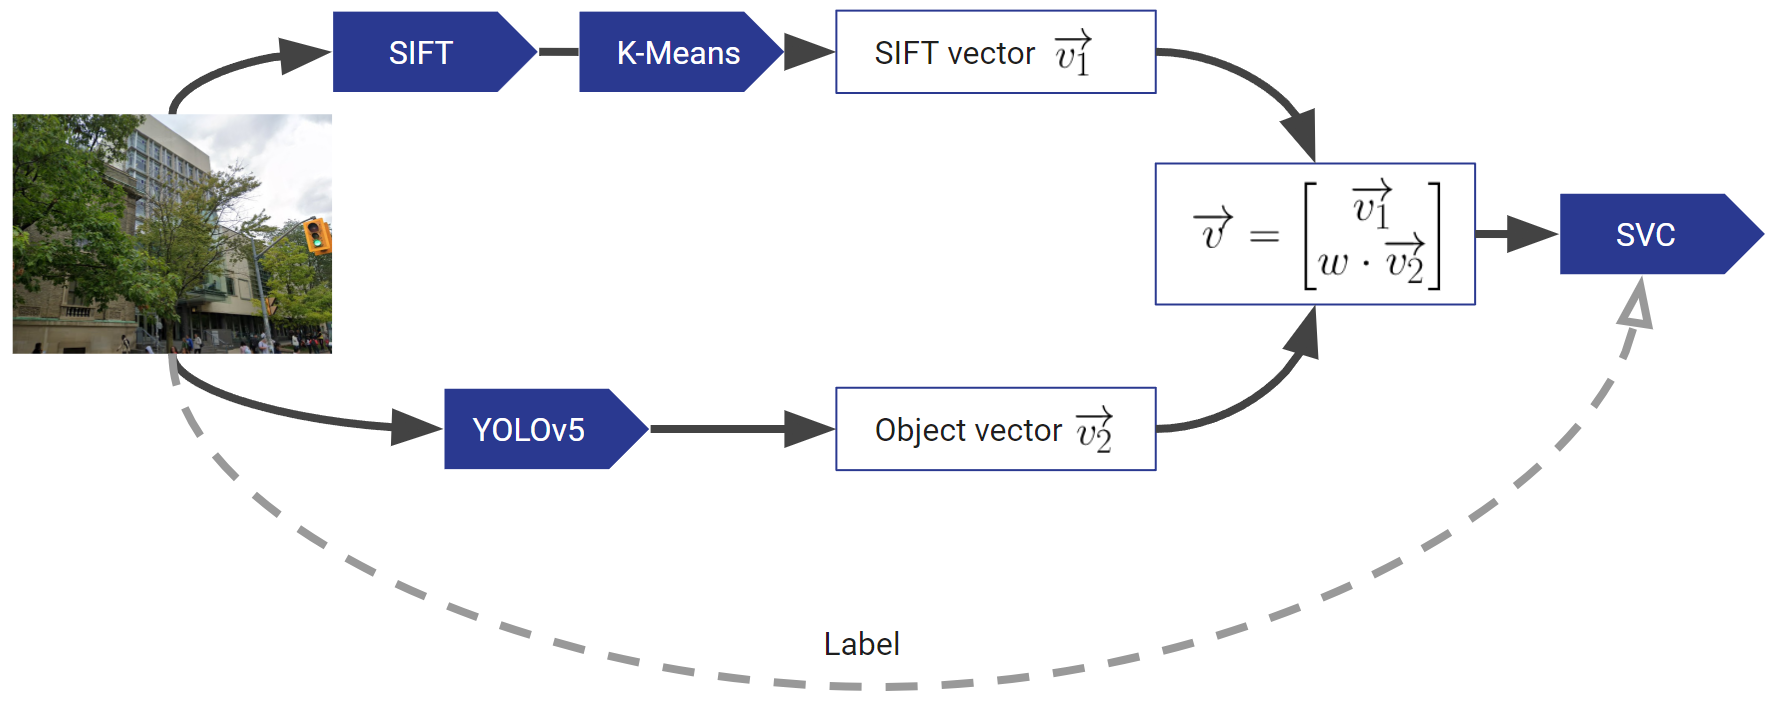
\includegraphics[width=0.45\textwidth]{fig_1.png}
    \caption{BoVW with Object Detection}
    \label{fig:1}
\end{figure}

\subsection{Optimization of Weighting Factor}

The choice of the weight factor has a significant impact on this extension. When the weighting factor is too small, object detection will barely influence the decision of the SVC. When the weighting factor is too large it will lead to overfitting.

We have written an automated program to conduct a large number of experiments with different weighting factors and to narrow down the searching range of the weighting factor. In the end, we found that the best performance was achieved with $w = 10$. The following tables show some of our test results for different weighting factor values. These accuracy improvements refer to the comparison with the primitive BoVW.

\begin{table}[ht]
    \centering
    \caption{Average Accuracy improvements (\%) (5 Rounds)}
    \begin{tabular}{|c|c|c|c|c|c|}
    \hline \textbf{\# of places} & $w = 1$ & $w = 10$ & $w = 20$ & $w = 30$ & $w = 40$\\
    \hline 50 & 0.0 & -0.4 & 0.4 & -0.8 & -1.2\\
    \hline 100 & 0.2 & 0.4 & -0.8 & -0.6 & -1.4\\
    \hline 200 & 0.0 & 1.6 & 0.8 & -0.1 & -1.1\\
    \hline
    \end{tabular}
\end{table}

\begin{table}[ht]
    \centering
    \caption{Average Accuracy improvements (\%) (10 Rounds)}
    \begin{tabular}{|c|c|c|c|c|c|}
    \hline \textbf{\# of places} & $w = 10$ & $w = 15$ & $w = 20$ & $w = 25$ & $w = 30$\\
    \hline 50 & 0.2 & -0.4 & -0.4 & -0.6 & -1.2\\
    \hline 100 & 2.5 & 2.5 & 2.1 & 1.6 & 0.8\\
    \hline 200 & 2.7 & 2.1 & 1.4 & 0.3 & -0.4\\
    \hline
    \end{tabular}
\end{table}

\section{RoNI Detection}

\textbf{Note:} This extension has been deprecated, as we found in our tests that it did not provide a performance increase, but rather led to a decrease in accuracy. This exploration is only briefly described here for discussion purposes.

\subsection{Overview}

Based on the primitive BoVW implementation, we found the algorithm performs poorly when there is a large proportion of the testing image is vegetation. So one direct attempt is to reduce the reliance on the descriptors for features of vegetation. Also, intuitively, as the objects like vehicles are moving now and then, descriptors for those variant object should be ignored for our location classification problem.

\begin{figure}[H]
    \centering
    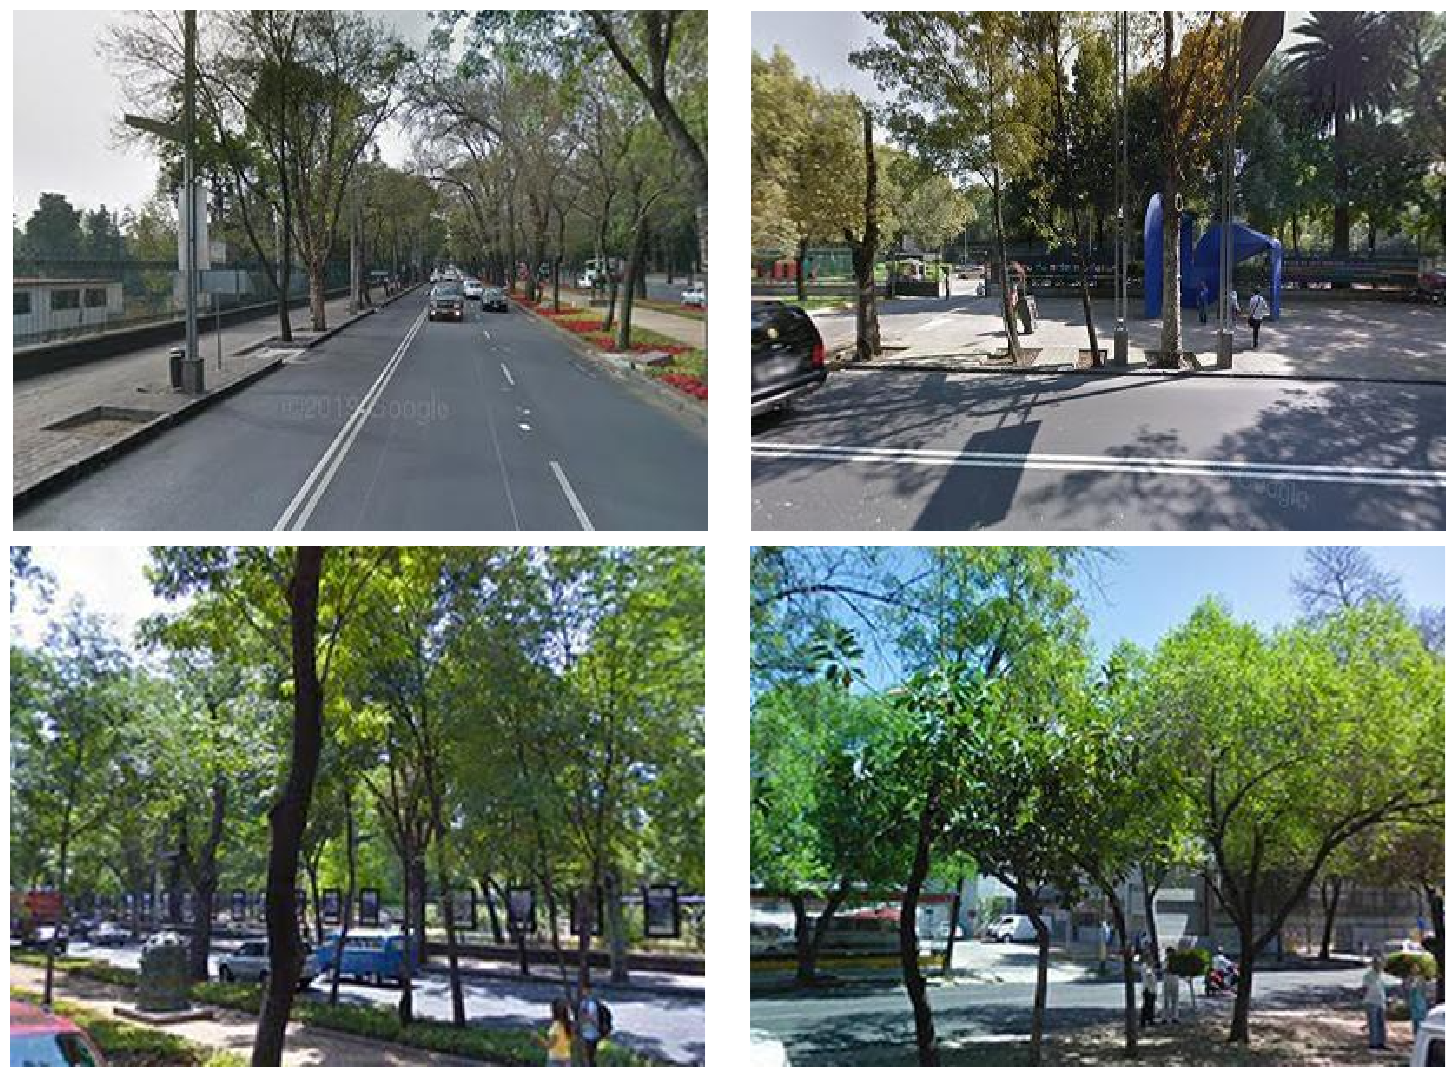
\includegraphics[width=0.45\textwidth]{fig_2.png}
    \caption{Two pairs of incorrectly matched locations}
    \label{fig:2}
\end{figure}

\subsection{Generating Vegetation Mask}

For vegetation region identification, we use a simple approach. First, we convert the image color space from RGB to HSV since HSV provides a more accurate description of color in different conditions. Then we just examine the area of the image that falls within our defined ``green'' HSV interval and use it as our vegetation mask.

\subsection{Moving Object Detection}

To detect moving objects, we again used the pre-trained YOLO model. We set the following moving objects, which are common outdoors, as targets.

\begin{verbatim}
    EXCLUDE_NAMES = set([
        'person',
        'bicycle',
        'motorbike',
        'car',
        'bus',
        'truck',
    ])
\end{verbatim}

YOLO generates a bounding box for each detected target object. We set the bounding box (rectangle) as the region of no interest.

\subsection{Result and Discussions}

Combine the RoNI masks from the previous two sections, we are able to create our final RoNI mask. It did ignore some of the feature points as we expected (as shown below\ref{fig:3}, the right figures show the result after feature filtering).

\begin{figure}[H]
    \centering
    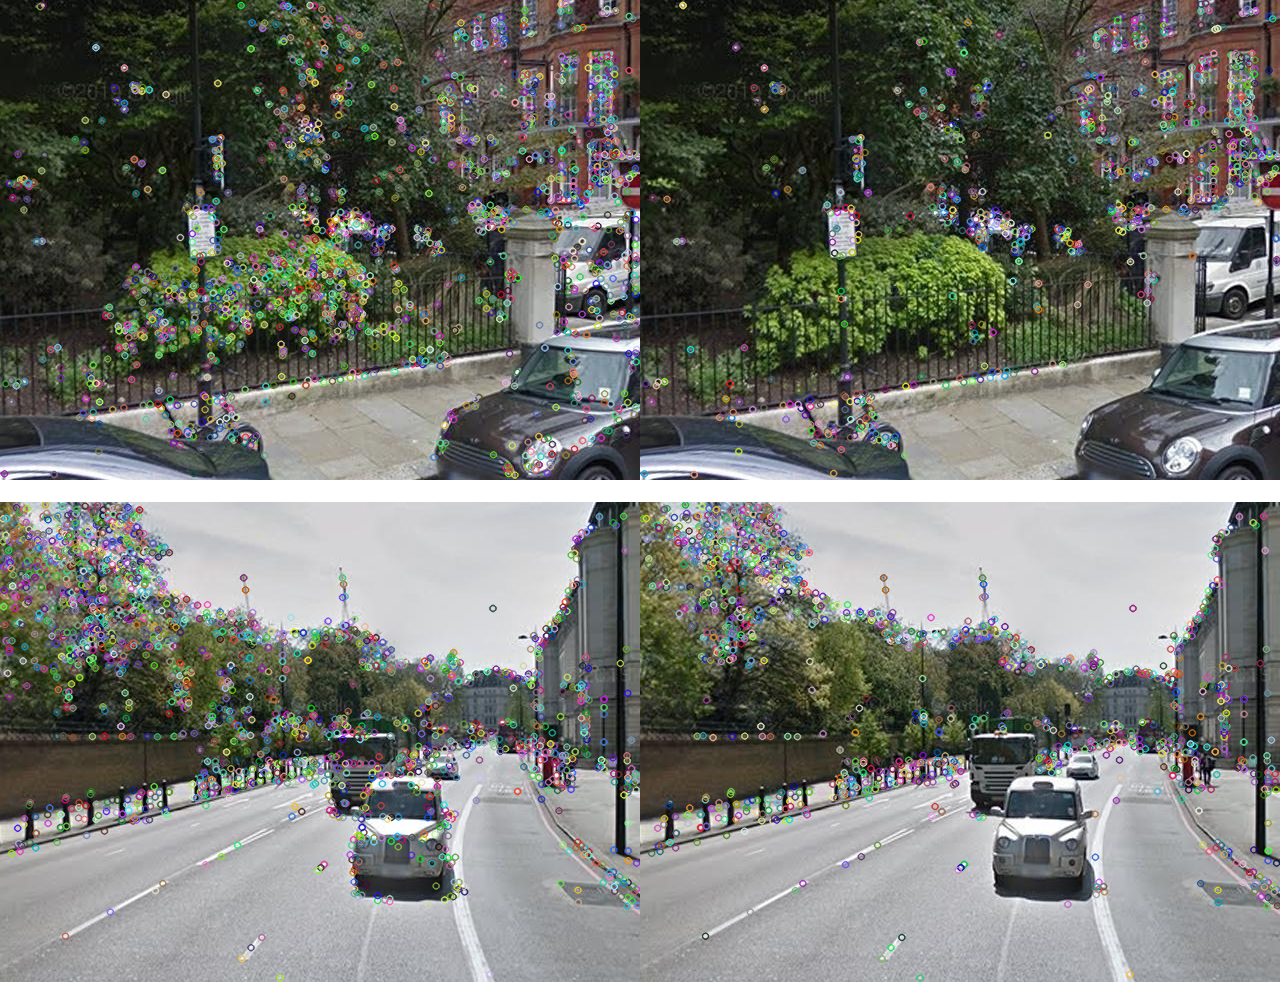
\includegraphics[width=0.45\textwidth]{fig_3.png}
    \caption{RoNI comparison}
    \label{fig:3}
\end{figure}

After testing, we found that while our RoNI detection appeared to work fine, it actually reduced the accuracy by 1\% to 2\%.

We have the following possible explanations for the performance drop:

\paragraph{Inaccurate RoNI masking}

First of all, our detection of vegetation areas is too simple to really identify all vegetation areas, especially those with yellowish colors. Secondly, we are using bounding boxes as our masks, which is also inaccurate. We probably should consider using instance segmentation models to find the actual RoNI.

\paragraph{Exclusion of valuable features}

For example, it is possible that similar features on cars could be used as a evidence for determining whether a scene is a road or not. Therefore removing the features on the car will result in a decrease in accuracy.

\section{Performance and Results}

\subsection{Dataset}

To test the performance of our baseline and extensions, we utilized the GSV-Cities dataset\cite{ali2022gsv}, which is specifically designed for tasks of VPR. This dataset is extensive, containing around 530,000 images from over 62,000 different locations. The variety of images, each taken from multiple angles and under various lighting and time conditions, makes it an ideal choice for VPR research.

In order to reduce the computational resources required for testing, we wrote data extraction programs that randomly selected locations from four cities, London, Boston, Chicago, and Osaka, to form the dataset. One random image from each location was used as the test data and the remaining images were used as the training data. To ensure the stability of the test, we filtered out the locations with too few images. In the following tests, there are on average 12 images per location.

\subsection{Performance}

To ensure that the tests were representative, we generated 100 different randomized test sets for different numbers of locations (50, 100, 200) using the method described above. We then tested our baseline algorithm and the extended algorithm with object detection ($w = 10$) on these data.

\begin{table}[ht]
    \centering
    \caption{Test Result (Baseline, 100 Rounds)}
    \begin{tabular}{|c|c|c|c|}
    \hline \textbf{\# of places} & \textbf{Accuracy(\%)} & \textbf{Training Time(s)} & \textbf{Testing Time(s)}\\
    \hline 50 & 78.92 & 55.94 & 3.96\\
    \hline 100 & 75.70 & 108.05 & 5.42\\
    \hline 200 & 70.88 & 210.74 & 8.43\\
    \hline
    \end{tabular}
\end{table}

\begin{table}[ht]
    \centering
    \caption{Test Result (Object Detection, $w = 10$, 100 Rounds)}
    \begin{tabular}{|c|c|c|c|}
    \hline \textbf{\# of places} & \textbf{Accuracy(\%)} & \textbf{Training Time(s)} & \textbf{Testing Time(s)}\\
    \hline 50 & 80.24 & 66.61 & 6.91\\
    \hline 100 & 76.98 & 127.23 & 9.06\\
    \hline 200 & 72.55 & 246.73 & 13.88\\
    \hline
    \end{tabular}
\end{table}


Compare the two results, there is a noticeable increase in accuracy. Specifically, the accuracy increased by 1.32\% for 50 places, 1.28\% for 100 places, and 1.66\% for 200 places.

It is worth noting that since it takes about two seconds to load the YOLOv5 model each time, and real applications do not need to load the model frequently, the percentage increase in test time is actually less than it appears.

We can see that our proposed extension is able to improve the accuracy of the model by an average of 1.42\% by adding only five words to the vocabulary, without significantly increasing the computational complexity. This shows the potential our model has for practical applications.

\subsection{The Deliverable}

To verify the feasibility of our model in the real world, we took around 12 photos at each of the 10 locations on the University of Toronto's St. George campus, trained a model based on this data. We used the model to build an online API and wrote a front-end website to invoke it. Since we did not have time to collect a large amount of data for accuracy testing, our model worked well in real-world testing, even if the time of day and weather were different from when the training set was collected.

\begin{figure}[H]
    \centering
    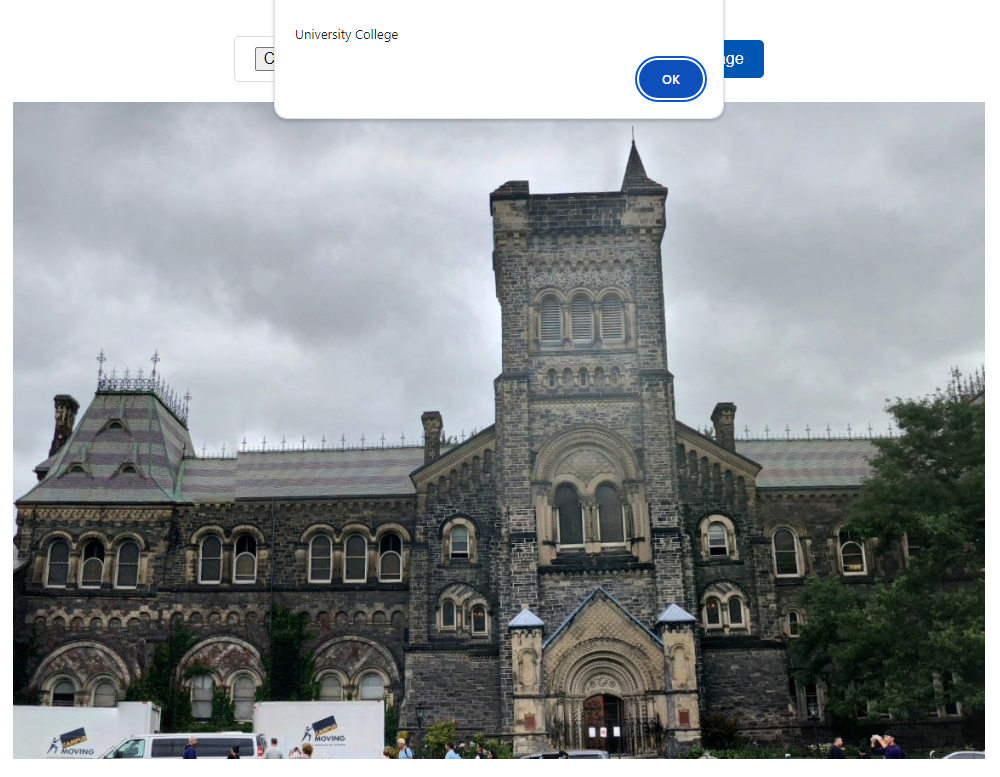
\includegraphics[width=0.45\textwidth]{fig_4.png}
    \caption{The Deliverable Web-page}
    \label{fig:4}
\end{figure}

\section{Conclusion and Future Potential}

Currently, our system only considers five different feature objects. Expanding this list to include more diverse and location-specific objects could further improve accuracy. For instance, incorporating the detection of unique building styles or other permanent urban features could provide more distinctive cues for place recognition.

In conclusion, this report discusses the application of BoVW to the VPR problem and presents two extensions on BoVW. Among them, feature object detection is shown to be able to improve the accuracy of the BoVW method with only a small increase in computational complexity, giving a new direction for BoVW optimization. In addition, we believe that further research into the causes of failure of proposed RoNI detection will also benefit VPR researches.

\bibliographystyle{plain}
\bibliography{references}

\end{document}